\documentclass[a4paper,UTF8]{article}
\usepackage{ctex}
\usepackage[margin=1.25in]{geometry}
\usepackage{ifpdf}
\usepackage{color}
\usepackage{graphicx}
\usepackage{amssymb}
\usepackage{amsmath}
\usepackage{amsthm}
\usepackage{enumerate}
\usepackage{bm}
\usepackage{hyperref}
\usepackage{pgfplots}
\usepackage{epsfig}
\usepackage{color}
\usepackage{tcolorbox}
\usepackage{mdframed}
\usepackage{lipsum}
\usepackage{framed}
\usepackage{setspace}

\newmdtheoremenv{thm-box}{myThm}
\newmdtheoremenv{prop-box}{Proposition}
\newmdtheoremenv{def-box}{定义}

\setlength{\evensidemargin}{.25in}
\setlength{\textwidth}{6in}
\setlength{\topmargin}{-0.5in}
\setlength{\topmargin}{-0.5in}
% \setlength{\textheight}{9.5in}
%%%%%%%%%%%%%%%%%%此处用于设置页眉页脚%%%%%%%%%%%%%%%%%%
\pgfplotsset{compat=1.18}
\usepackage{fancyhdr}                                
\usepackage{lastpage}                                           
\usepackage{layout}                                             
\footskip = 12pt 
\pagestyle{fancy}                    % 设置页眉                 
\lhead{2024年秋季}                    
\chead{数字信号处理}                                                
% \rhead{第\thepage/\pageref{LastPage}页} 
\rhead{作业二}                                                                                               
\cfoot{\thepage}                                                
\renewcommand{\headrulewidth}{1pt}  			%页眉线宽，设为0可以去页眉线
\setlength{\skip\footins}{0.5cm}    			%脚注与正文的距离           
\renewcommand{\footrulewidth}{0pt}  			%页脚线宽，设为0可以去页脚线

\makeatletter 									%设置双线页眉                                        
\def\headrule{{\if@fancyplain\let\headrulewidth\plainheadrulewidth\fi%
\hrule\@height 1.0pt \@width\headwidth\vskip1pt	%上面线为1pt粗  
\hrule\@height 0.5pt\@width\headwidth  			%下面0.5pt粗            
\vskip-2\headrulewidth\vskip-1pt}      			%两条线的距离1pt        
 \vspace{6mm}}     								%双线与下面正文之间的垂直间距              
\makeatother  

%%%%%%%%%%%%%%%%%%%%%%%%%%%%%%%%%%%%%%%%%%%%%%
\numberwithin{equation}{section}
%\usepackage[thmmarks, amsmath, thref]{ntheorem}
\newtheorem{myThm}{myThm}
\newtheorem*{myDef}{Definition}
\newtheorem*{mySol}{Solution}
\newtheorem*{myProof}{Proof}
\newtheorem*{myRemark}{备注}
\renewcommand{\tilde}{\widetilde}
\renewcommand{\hat}{\widehat}
\newcommand{\indep}{\rotatebox[origin=c]{90}{$\models$}}
\newcommand*\diff{\mathop{}\!\mathrm{d}}

\usepackage{multirow}

%--

%--
\begin{document}

\title{数字信号处理\\
    作业二}
\author{田永铭\, 221900180}
\maketitle

\section*{作业提交注意事项}
\begin{tcolorbox}
    \begin{enumerate}
       \item[(1)] 本次作业提交截止时间为~\textcolor{red}{\textbf{2024/12/11  23:59:59}}，截止时间后不再接收作业；
        \item[(2)] 作业提交方式：使用此~LaTex~模板书写解答，不允许使用手写图片替代~LaTex~格式解题过程，只需提交编译生成的~pdf~文件，将~pdf~文件发送至邮箱：779652674@qq.com；
        \item[(3)] pdf 文件命名方式：学号-姓名-作业号-v版本号, 例~ 1900000-张三-1-v1；如果需要更改已提交的解答，请在截止时间之前提交新版本的解答，并将版本号加一；
        \item[(4)] 作业提交规范占5分，未按照要求提交作业，或~pdf~命名方式不正确，将会被扣除此部分分数。
    \end{enumerate}
\end{tcolorbox}

\newpage
\section{[20pts]}
解差分方程（$n\ge 0$），并指出其零输入响应、零状态响应、自由响应、强迫响应各分量。（假定系统为因果系统）
$$y[n]+3y[n-1]+2y[n-2]=0,y[-1]=2,y[-2]=1$$

\begin{framed}
	   	解：
   \begin{itemize}
		\item \textbf{解方程：}
		
	特征方程为:
	\[
	\alpha^2 + 3\alpha + 2 = 0,
	\]
	解得：$\alpha_1 = -1,\alpha_2 = -2$.
	所以齐次解为$y_h = A(-1)^n + B(-2)^n$.
	由于方程输入为$0$,所以特解为$y_p = 0$.所以完全解为$y = y_h + y_p = A(-1)^n + B(-2)^n$.
	利用原式可以得到: $y[0] + 3y[-1] + 2y[-2] = 0$, 以及 $y[1]+3y[0] + 2y[-1] = 0$, 所以$y[1] = 20, y[0] = -8.$因此
	$$
	\begin{cases}
		A(-1)^0+ B(-2)^0 = -8,\\
		A(-1)^1+ B(-2)^1 = 20,\\
	\end{cases}
	$$解得：$A = 4, B = -12$.
	因此完全解为$y = 4\cdot(-1)^n - 12\cdot(-2)^n(n \geq 0).$
	
	\item \textbf{各个部分:}
	
	由于系统原方程本身就没有外部驱动，所以\textbf{零输入响应}和\textbf{自由响应}相等，均等于$4\cdot(-1)^n - 12\cdot(-2)^n$;\textbf{零状态响应}和\textbf{强迫响应}相等，均等于$0$.
   \end{itemize}
\end{framed}


\newpage
\section{[40pts]}
求下图中所示对称周期矩形信号的傅里叶级数（三角形式与指数形式）。
\begin{figure}[htbp]
	\centering
	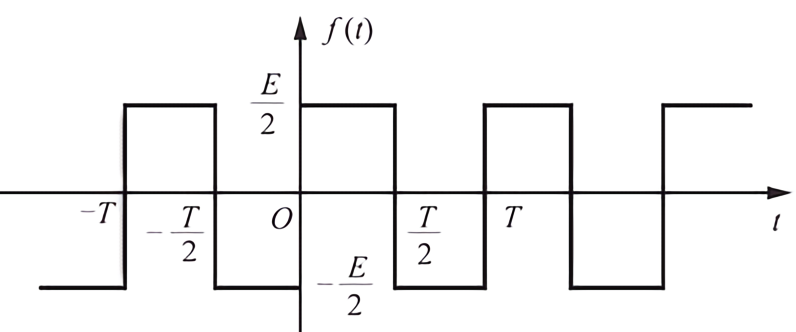
\includegraphics[scale=0.3]{image1.png}
\end{figure} 

\begin{framed}
	解：
	\begin{enumerate}[(1)]
		\item 三角形式：
		因为是奇信号，所以只有$b_n$不为0.
		\begin{align*}
			b_n &= \frac{2}{T}\int_{0}^{T}x(t)sin(n\omega t)dt\\
			&= \frac{2}{T}(\int_{0}^{\frac{T}{2}}\frac{E}{2}sin(n\omega t)dt - \int_{\frac{T}{2}}^{T}\frac{E}{2}sin(n\omega t)dt)\\
			&= \frac{E}{-n\omega T}\cdot([cosn\omega t]|_{0}^{\frac{T}{2}} - [cosn\omega t]|_{\frac{T}{2}}^{T})\\
			&= \frac{E}{n\pi}(1-cosn\pi)
		\end{align*}
		所以三角形式傅里叶级数(只有$n$为奇数的时候有)为：
		$x(t) = \sum\limits_{n = 1,3,5\cdots}^{\infty} \frac{2E}{n\pi}sinn(\frac{2\pi}{T}) t$.
		\item 指数形式：
		由$X_n$和$a_n$和$b_n$的关系可得：
		$X_n = \frac{1}{2}a_n-\frac{j}{2}b_n = \frac{-jE}{2n\pi}(1-cosn\pi)$.
		
		或者直接计算:
		
		\begin{align*}
			X_n &= \frac{1}{T}\int_{0}^{T}x(t)e^{-njwt}\\
			&= \frac{1}{T}(\int_{0}^{\frac{T}{2}}\frac{E}{2}e^{-njwt}dt - \int_{\frac{T}{2}}^{T}\frac{E}{2}e^{-njwt}dt)\\
			&= \frac{E}{-j4n\pi}\cdot([e^{-njwt}]|_{0}^{\frac{T}{2}} - [e^{-njwt}]|_{\frac{T}{2}}^{T})\\
			&= \frac{-jE}{2n\pi}(1-e^{-nj\pi})
		\end{align*}
		
		由于$e^{-nj\pi} = cosn\pi$,所以两种方法结果一致。
		
		所以指数形式傅里叶级数为：
		$x(t) = \sum\limits_{n = \pm1,\pm3\cdots}^{\pm\infty}\frac{-jE}{n\pi}e^{jn(\frac{2\pi}{T})t} $.
		
	\end{enumerate}
\end{framed}





\newpage
\section{[40pts]}
求下图所示锯齿脉冲与单周正弦脉冲的傅里叶变换。
\begin{figure}[htbp]
	\centering
	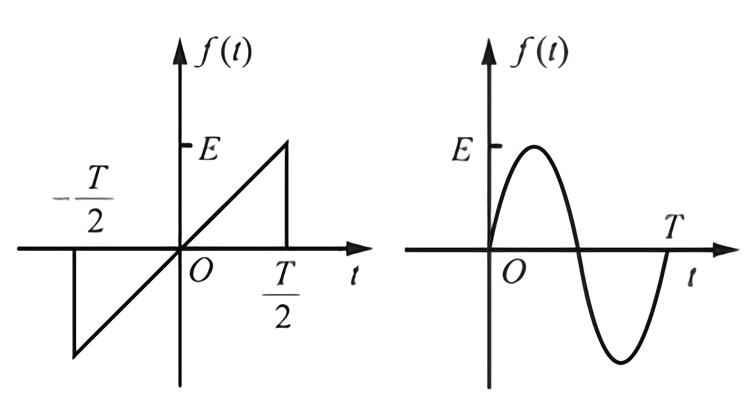
\includegraphics[scale=0.3]{image2.png}
\end{figure} 

\begin{framed}
	解：
	\begin{enumerate}[(1)]
		\item 锯齿脉冲：	
		
		\textbf{当$\omega \neq 0$时}：
		\begin{align*}
			X(jw) &= \int_{-\infty}^{+\infty}x(t)e^{-jwt}dt\\
			&= \int_{-\frac{T}{2}}^{\frac{T}{2}}\frac{2E}{T}t\cdot e^{-jwt}dt\\
			&= \frac{2E}{-j\omega T}\int_{-\frac{T}{2}}^{\frac{T}{2}}tde^{-j\omega t}\\
			& = \frac{2E}{-j\omega T}([te^{-j\omega t}]_{-\frac{T}{2}}^{\frac{T}{2}} - \int_{-\frac{T}{2}}^{\frac{T}{2}}e^{-jwt}dt)\\
			&= \frac{2E}{-j\omega T}(T\cdot cos\frac{\omega T}{2} - \frac{e^{-jwt}|_{-\frac{T}{2}}^{\frac{T}{2}}}{-j\omega})\\
			&= j\frac{2E}{\omega}[cos(\frac{\omega T}{2}) - Sa(\frac{\omega T}{2})]
		\end{align*} 
		\textbf{当$\omega = 0$时：}
		
		$X(jw) = \int_{-\frac{T}{2}}^{\frac{T}{2}}\frac{2E}{T}tdt = 0$.
		\item 
		记$\omega_1 = \frac{2\pi}{T}$,则：
		
		\textbf{当$\omega \neq \omega_1$时：}
		\begin{align*}
			X(jw) &= \int_{-\infty}^{+\infty}x(t)e^{-jwt}dt\\
			&= \int_{0}^{T}Esin(\frac{2\pi}{T}t)\cdot e^{-jwt}dt\\
			&= \frac{E}{2j}(\int_{0}^{T}e^{(j\omega_1-j\omega)t}dt - \int_{0}^{T}e^{(-j\omega_1-j\omega)t}dt)\\
			&= \frac{E}{2j}(\frac{e^{-j\omega T} - 1}{j\omega_1-j\omega} - \frac{e^{-j\omega T} - 1}{-j\omega_1-j\omega})\\
			&= \frac{E\omega_1}{\omega_1^2-\omega^2}(1-e^{-jwT})\\
			&= j\frac{2E\omega_1}{\omega_1^2-\omega^2}sin(\frac{\omega T}{2})e^{-j\frac{\omega T}{2}}\quad(\omega_1 = \frac{2\pi}{T})
		\end{align*}
		
		\textbf{当$\omega = \omega_1$时：}
		
		$X(jw) = \frac{ET}{2j}\quad(\omega_1 = \frac{2\pi}{T})$.
	\end{enumerate}
\end{framed}


\end{document} 